\section{Introduction}
Using a control contact draped over \ac{hBN} we demonstrated strong evidence for a normal mode on that exists purely on the hinge or side of the \ac{FTS} crystal\cite{Gray2019}. Recent works have called into question the exact topological nature of \ac{FTS} claiming the crystal is not a topological insulator but rather a topological semi-metal with buried Dirac nodes. In light of this it is crucial to obtain evidence with more experimental techniques to better understand the nature of the topology in the \ac{FTS} system. Indeed, the underlying physics which predicts the helical hinge mode also predicts the same mode to manifest as a bias-independent conductance plateau in a differential conductance measurement rather than the previously observed zero-bias conductance peak. To accomplish this, we investigate the effect edge quality has on the topological characteristics of \ac{FTS} as it has been previously shown that the quality of the crystal edge can have a drastic effect on its transport characteristics \todo{cite Andrea's work on different transport characteristics of graphene}. We find that when tunneling measurements are performed across pristine, high-symmetry crystalline edges bias-independent conductance plateaus are observed for biases below the superconducting gap energy while ``rough" edges do not exhibit such plateaus. Furthermore, these plateaus are consistent with \acl{PAR}.

\section{Observation of Bias-Independent Conductance Plateau}
The tunneling conductance of a normal-metal/superconductor interface can be modeled by assuming an delta-function potential barrier at the interface characterized by a strength parameter $Z$, i.e., the \ac{BTK} method. An in-depth discussion and pseudo code for performing these simulations can be found in \ref{app:ARfit}], however we will take some of the main results of these calculations for discussions here. The \ac{BTK} method on a standard \ac{BCS} s-wave superconductor predicts a bias-independent conductance plateau only when the strength of the potential barrier between the normal-metal and superconductor is exactly zero. Even slight deviations from a zero-strength barrier result in significant dips around zero-bias, thus observing \ac{PAR} is exceedingly rare and typically only occurs only in extremely clean materials \todo{cite klein paper}. Therefore when \ac{PAR} is observed in a system it is usually due to an underlying mechanism which causes the incoming carriers to ignore the barrier completely; these mechanisms include forbidden backscattering due to topological spin-momentum locked bands and majorana zero-mode assisted tunneling, among others. \ac{PAR} has three unique identifiers in a differential conductance spectrum: a perfectly flat plateau, the plateau is at twice the conductance of the normal state, and the plateau extends out to the superconducting energy gap.\par
\begin{figure}[h]
    \centering
    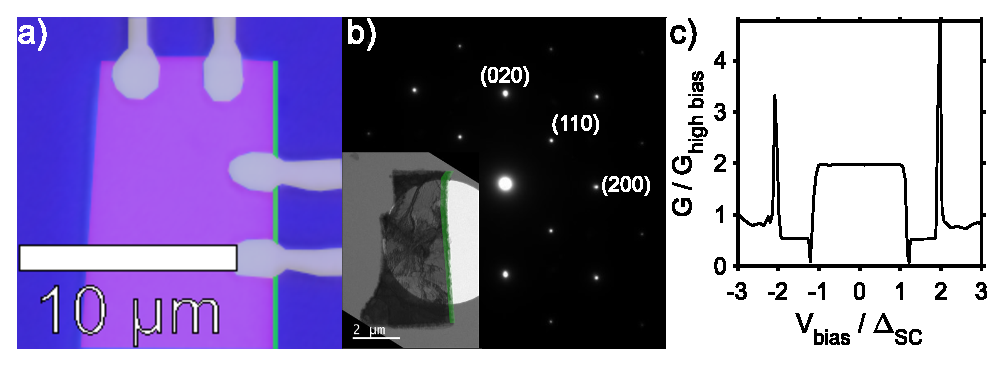
\includegraphics[width = \textwidth]{Chap4/Figures/DeviceFab.eps}
    \caption{a) False color optical image of a representative device with a straight (100) edge which is highlighted in green. b) \ac{TEM} diffraction pattern demonstrating the (100) edge. Inset shows the flake measured as well as the diffraction aperture. c) Base temperature differential conductance curve.}
    \label{fig:PARDeviceFab}
\end{figure}
\todo{Make Edge vs Plateau figure}
This bias-independent conductance plateau is observed in other devices with straight edges, however when performing tunneling experiments on ``rough" edges (i.e. edges that are not straight) the differential conductance does not show a plateau at low-biases (Fig \todo{fig ref}). This suggests that the \ac{PAR} in this system is sensitive to the local contact conditions or the contact to the bulk superconductivity is highly-sensitive to the details of the contact. In the latter case, the \ac{PAR} is not affected by the local contact conditions but the signal is drowned out among a much larger supercurrent when better contact is made to the superconducting bulk. 
\begin{figure}[h]
    \centering
    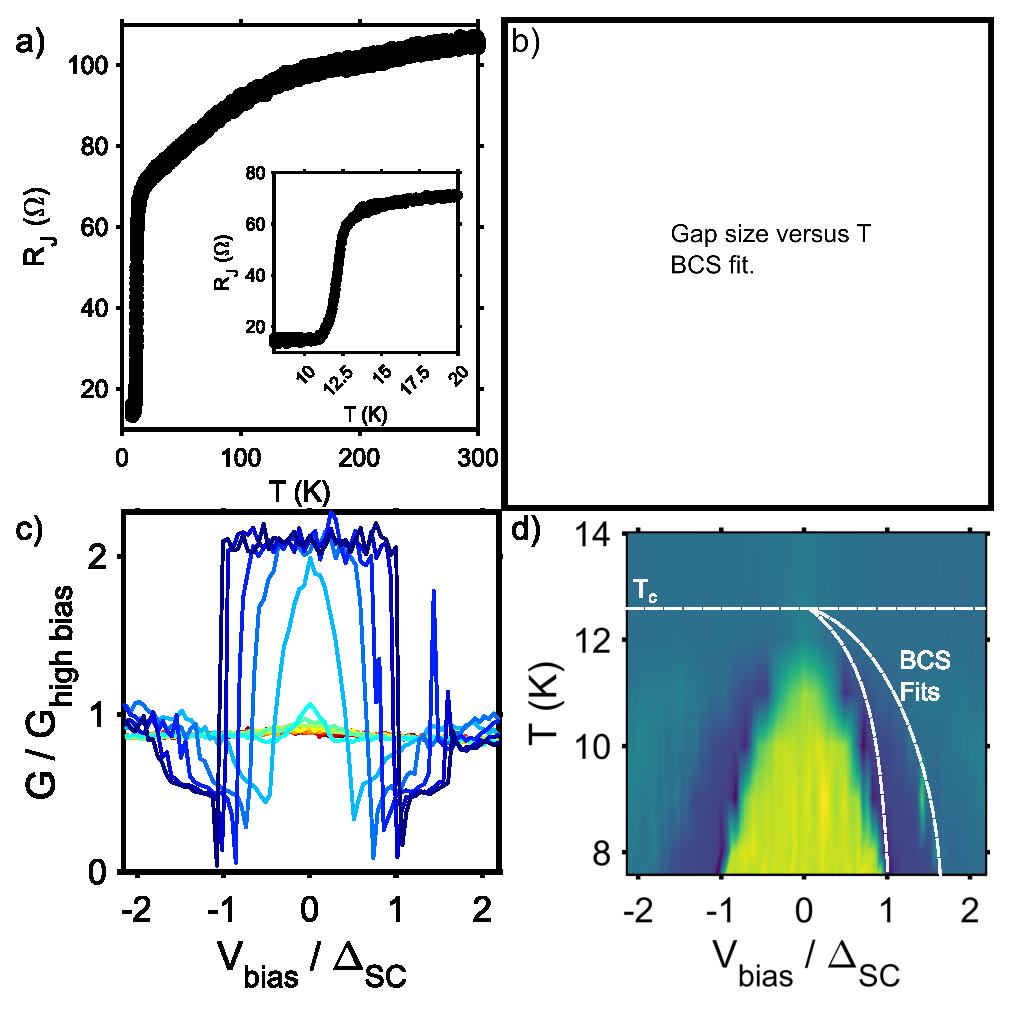
\includegraphics[width = \textwidth]{Chap4/Figures/Temperature.eps}
    \caption{Caption}
    \label{fig:PARTemp}
\end{figure}

\section{Magnetic Field Dependence}
Topological materials are generally highly-sensitive to an external magnetic field, depending on the direction that the field is applied. Indeed, the Dirac surfaces states that are a key signature of a topological bulk are protected via time-reversal symmetry. It follows that if time-reversal symmetry is lifted via a magnetic field, any Dirac nodes that are aligned (the plane perpendicular to the spin-momentum locking determines the ``direction" of the cone) along the magnetic field will lose their topological protection. In contrast, if the Dirac node is perpendicular to the magnetic field, the node will simply shift up or down in energy but the node will keep its topological protection. In this manner, if the \ac{PAR} is caused by forbidden backscattering due to topological bands we expect highly anisotropic responses to different directions of applied magnetic field. While this seems to be the case in \ac{FTS} (shown in Fig \ref{fig:PARField}) we must be careful to differentiate the response of the \ac{PAR} from that of the bulk superconductor. Even though the upper critical field of \ac{FTS} is around $35 T$ \todo{cite field work} the bulk superconducting response of \ac{FTS} flakes is quite anisotropic, even below $9 T$ \cite{zalic2019}. When applying a magnetic field parallel with the hinge being measured (the a-axis of the material), the \ac{PAR} remains completely unaffected up to $5 T$. However, when the field is rotated to the c-axis of the crystal the \ac{PAR} seems to collapse quite rapidly which would give credence to a topological origin as discussed earlier. 
\begin{figure}[h]
    \centering
    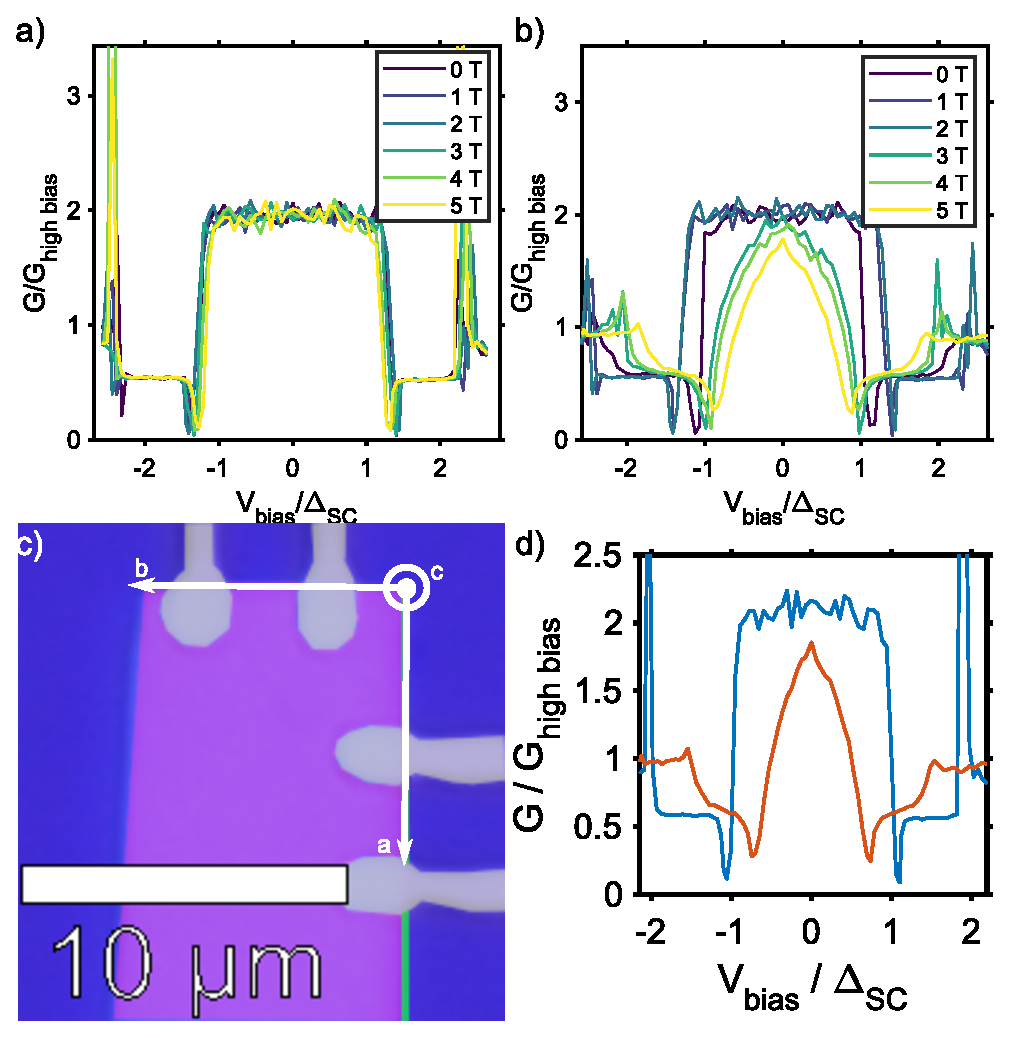
\includegraphics[width = \textwidth]{Chap4/Figures/MagneticField.eps}
    \caption{Caption}
    \label{fig:PARField}
\end{figure}
\section{Conclusion}
In this work we expanded upon the methods used in Chapter . When contacting straight, crystallographic edges we observe \acl{PAR} while contacts on ``rough" edges show normal \acl{AR} spectra. 